%%%%%%%%%%%%%%%%%%%%%%%%%%%%%%%%%%%%%%%%%
% Structured General Purpose Assignment
% LaTeX Template
%
% This template has been downloaded from:
% http://www.latextemplates.com
%
% Original author:
% Ted Pavlic (http://www.tedpavlic.com)
% Modified by:
% Jaime Dantas (https://jaimedantas.com)
%
% Note:
% The \lipsum[#] commands throughout this template generate dummy text
% to fill the template out. These commands should all be removed when 
% writing assignment content.
%
%%%%%%%%%%%%%%%%%%%%%%%%%%%%%%%%%%%%%%%%%

%----------------------------------------------------------------------------------------
%	PACKAGES AND OTHER DOCUMENT CONFIGURATIONS
%----------------------------------------------------------------------------------------

\documentclass{article}
\usepackage{fancyhdr} % Required for custom headers
\usepackage{lastpage} % Required to determine the last page for the footer
\usepackage{extramarks} % Required for headers and footers
\usepackage{graphicx} % Required to insert images
\usepackage{lipsum} % Used for inserting dummy 'Lorem ipsum' text into the template
\usepackage[utf8]{inputenc}
\usepackage[english]{babel}
\usepackage[]{biblatex}
\addbibresource{sample.bib}
\usepackage{hyperref}
\usepackage{amsmath}
\usepackage[most]{tcolorbox}
\usepackage{fontawesome}
\usepackage{tikz}
\usetikzlibrary{shapes.geometric}
\usepackage{enumerate}
\usepackage[ruled,vlined]{algorithm2e}
\usepackage{caption}
\usepackage[framed,autolinebreaks,useliterate]{mcode}
\usepackage{multicol}


% better for typesetting
\newcommand{\vect}[1]{\mathbf{#1}} % or \bm
\newcommand{\matr}[1]{\mathbf{#1}} % or \bm


%chart and draw
\tikzstyle{startstop} = [rectangle, minimum width=1cm, minimum height=1cm,text centered, draw=black, fill=white!30]

%tree

\tikzset{
  treenode/.style = {align=center, inner sep=0pt, text centered,
    },
  arn_n/.style = {treenode, rectangle, black, text centered, draw=black,
     thick, text width=6.5em, minimum height=2.5em, minimum width=6.5em},
  arn_r/.style = {treenode, circle, black, draw=black, 
    text width=1.5em,  thick, text width=3.5em, minimum height=1.5em, minimum width=3.5em},
  arn_x/.style = {treenode, rectangle, draw=black,
    minimum width=0.5em, minimum height=0.5em}
}

% Margins
\topmargin=-0.45in
\evensidemargin=0in
\oddsidemargin=0in
\textwidth=6.5in
\textheight=9.0in
\headsep=0.25in 

\linespread{1} % Line spacing

% Set up the header and footer
\pagestyle{fancy}
\chead{\textmd{\hmwkClass} \textemdash \textmd{ \hmwkTitle}} % Top center header
\rhead{\firstxmark} % Top right header
\lfoot{\lastxmark} % Bottom left footer
\cfoot{} % Bottom center footer
\cfoot{Page\ \thepage\ of\ \pageref{LastPage}} % Bottom right footer
\renewcommand\headrulewidth{0.4pt} % Size of the header rule
\setlength\parindent{0pt} % Removes all indentation from paragraphs

%----------------------------------------------------------------------------------------
%	DOCUMENT STRUCTURE COMMANDS
%	Skip this unless you know what you're doing
%----------------------------------------------------------------------------------------

% Header and footer for when a page split occurs within a problem environment
\newcommand{\enterProblemHeader}[1]{
\nobreak\extramarks{#1}{#1}\nobreak
\nobreak\extramarks{#1}{#1}\nobreak
}

% Header and footer for when a page split occurs between problem environments
\newcommand{\exitProblemHeader}[1]{
\nobreak\extramarks{#1}{#1}\nobreak
\nobreak\extramarks{#1}{}\nobreak
}

\setcounter{secnumdepth}{0} % Removes default section numbers
\newcounter{homeworkProblemCounter} % Creates a counter to keep track of the number of problems

\newcommand{\homeworkProblemName}{}
\newenvironment{homeworkProblem}[1][Problem \arabic{homeworkProblemCounter}]{ % Makes a new environment called homeworkProblem which takes 1 argument (custom name) but the default is "Problem #"
\stepcounter{homeworkProblemCounter} % Increase counter for number of problems
\renewcommand{\homeworkProblemName}{#1} % Assign \homeworkProblemName the name of the problem
\section{\homeworkProblemName} % Make a section in the document with the custom problem count
\enterProblemHeader{} % Header and footer within the environment
}{
\exitProblemHeader{} % Header and footer after the environment
}


\newcommand{\homeworkSectionName}{}
\newenvironment{homeworkSection}[1]{ % New environment for sections within homework problems, takes 1 argument - the name of the section
\renewcommand{\homeworkSectionName}{#1} % Assign \homeworkSectionName to the name of the section from the environment argument
\subsection{\homeworkSectionName} % Make a subsection with the custom name of the subsection
\enterProblemHeader{} % Header and footer within the environment
}{
\enterProblemHeader{} % Header and footer after the environment
}
   
%----------------------------------------------------------------------------------------
%	NAME AND CLASS SECTION
%----------------------------------------------------------------------------------------
\newcommand{\hmwkTitle}{Final Project - Group 4} % Assignment title
\newcommand{\hmwkDueDate}{Sunday,\ December\ 20,\ 2020} % Due date
\newcommand{\hmwkClass}{EECS\ 4404/5327} % Course/class
\newcommand{\hmwkClassInstructor}{Dr. Ruth Urner} % Teacher/lecturer
\newcommand{\hmwkAuthorName}{Jaime Dantas} % Your name


%----------------------------------------------------------------------------------------
%	TITLE PAGE
%----------------------------------------------------------------------------------------

\title{

\includegraphics[scale=0.35]{lassonde.png}\\
\large{Department of Electrical Engineering \& Computer Science}\\

\vspace{1in}
\Huge{\textbf{\hmwkTitle}}\\
\vspace{0.1in}
\Large{\textbf{Course:} \hmwkClass}\\
\vspace{0.1in}
\Large{\textbf{Instructor:} \hmwkClassInstructor }\\
\vspace{0.1in}
\Large{\textbf{Due Date:} \hmwkDueDate}\\

\vspace{1in}
}

\author{
    \begin{tabular}{@{}ll@{}}
    \textbf{Name} & \textbf{Student \#} \\
    \hline
    Baoqi Yu & 0 \\
    David Mounes        & 0                          \\
    Jaime Dantas       & 0     \\
    Matthew Tolentino         & 0                           \\
    Minghong Xu         & 0                          \\
    Nizwa Javed        & 0                          \\
    Thomas Lykouras        & 0                          \\
    Yiming Shao         & 0                  \\        
    Umer Qudrat         & 0                          
    \end{tabular}
}

\date{\large{\today}} % Insert date here if you want it to appear below your name

%----------------------------------------------------------------------------------------

\begin{document}

\maketitle
\thispagestyle{empty}

\newpage

% --------------------- Section 1
\setcounter{page}{1}
\begin{homeworkProblem}[Planning and execution]
In order to better organize the workflow of the project, we created a project board on GitHub to keep track of all tasks involved. We split the project into 21 distinct tasks, and some of the tasks can be seen in the left picture of figure \ref{fig1}.
\\
\begin{minipage}{\textwidth}
\centering
    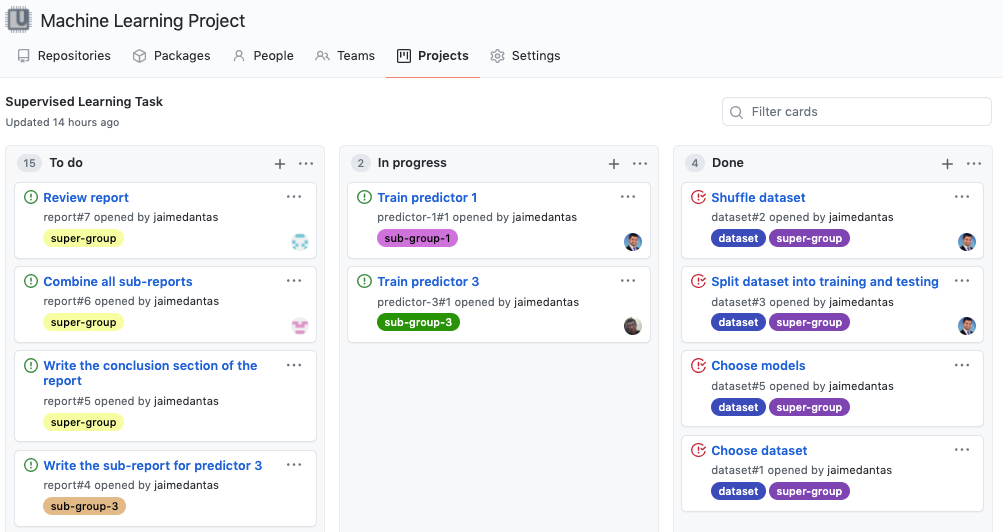
\includegraphics[width=0.495\textwidth]{board.png}
    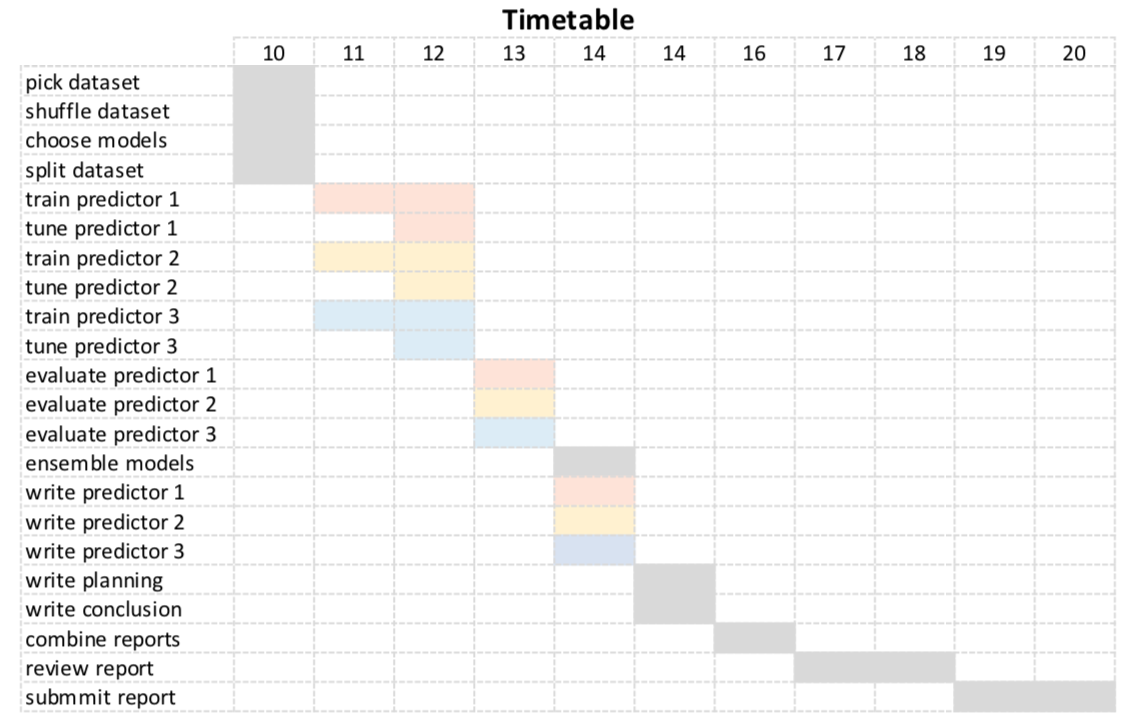
\includegraphics[width=0.47\textwidth]{timetable.png}
 \captionof{figure}{Project's task board on GitHub on the left and project's timetable on the right. Publicly available in \url{https://github.com/orgs/EECS-4404/projects/1}.}
 \label{fig1}
\end{minipage}
\\
A repository for each predictor was created on GitHub, and a timetable (left picture of figure \ref{fig1}) was followed. We split the super-group into 3 sub-groups as shown below.
\begin{center}
\begin{tabular}{@{}lll@{}}
\textbf{Sub-group 1} & \textbf{Sub-group 2} & \textbf{Sub-group 3}\\
\hline
Jamie Dantas &	Minghong Xu	&Nizwa Javed\\
Matthew Tolentino &	Baoqi Yu &	Thomas Lykouras                         \\
David Mounes &	Yiming Shao	 & Umer Qudrat  
\end{tabular}
\end{center}
Each sub-group trained a different predictor. Additionally, the remaining tasks were equally distributed among everyone. Several Zoom calls were made to discuss the project, and a Discord channel was created for discussion. 
\end{homeworkProblem}
% --------------------- Section 1a
\begin{homeworkProblem}[Dataset]
The dataset chosen was the \href{http://archive.ics.uci.edu/ml/datasets/Electrical+Grid+Stability+Simulated+Data+}{Electrical Grid Stability Simulated Dataset} from the UCI Repository \cite{UCI}. It is a binary classification problem with 13 real inputs that represents simulations of stability of a given electrical grid, and it has 10,000 data points.
\begin{multicols*}{2}
\begin{minipage}[t]{0.44\textwidth}
\centering
    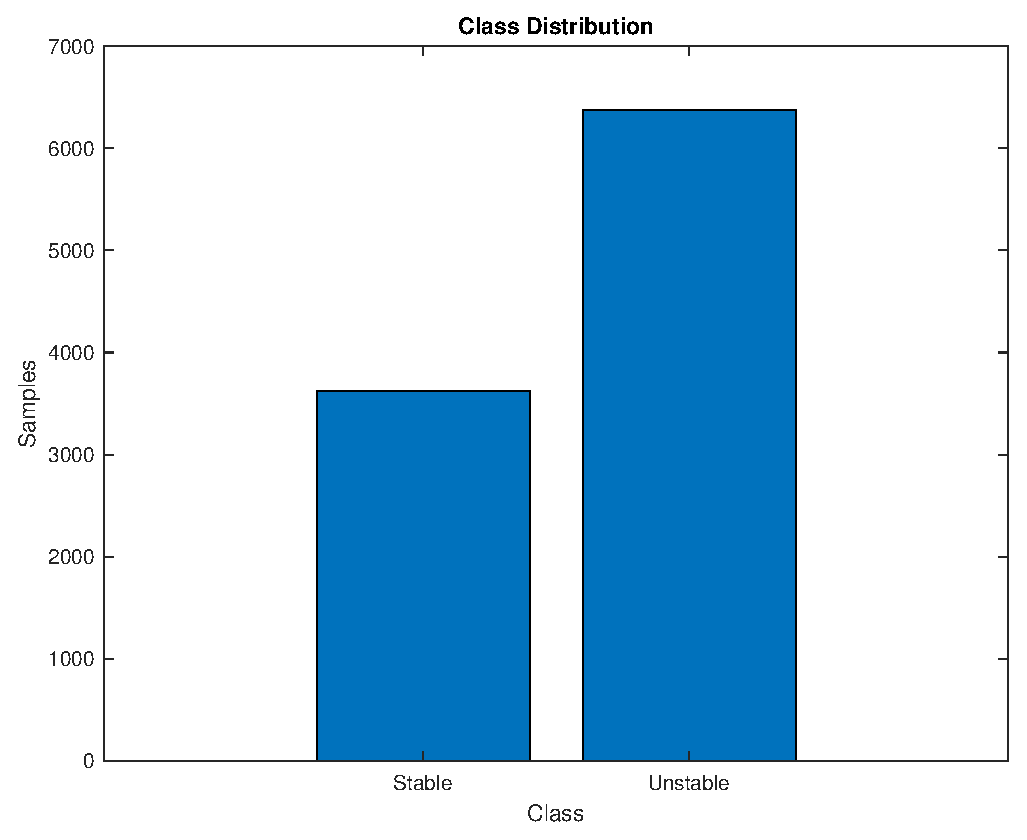
\includegraphics[width=1\linewidth]{bar_class.eps}
 \captionof{figure}{Class distribution of dataset. Publicly available in \url{https://github.com/EECS-4404/dataset}.}
 \label{dataset}
\end{minipage}
\\
\\
We performed a data pre-processing on the dataset to replace the class label "stable" and "unstable" to 1 and -1, respectively. The last input "stab" was removed since it contains the same information as the class label (stable if negative, unstable otherwise). Since this dataset is imbalanced, as shown in the figure \ref{dataset}, we used the F1-score for measuring the performance of the models. After pre-processing the dataset, we split it into a training dataset, with 80\% of the data points, and a testing dataset, with 20\% of the data points. The dataset was also shuffled. All the three predictors used the same data for training and testing. 
\end{multicols*}
\end{homeworkProblem}
\clearpage
% --------------------- Section 2
\begin{homeworkProblem}[Predictor \#1: feed-forward neural network]
The first predictor we trained was the feed-forward neural network. We used MATLAB for creating and tuning a pattern recognition neural network (\textit{patternnet}). First, we transformed the last column of the dataset, i.e., the class label +1/-1, into two new columns filled with 1 in the index that represents the class and 0 otherwise $\left[ \begin{smallmatrix}\text{stable}&  \text{unstable}\end{smallmatrix}\right]$. Then, we tried a different set of combinations of hidden layers and neurons always aiming to simplicity over complexity. This process resulted in the creation of a neural network with two hidden layers with 36 and 24 neurons, respectively, as shown in the figure \ref{neural}. 
\\
\\
\begin{minipage}{\textwidth}
\centering
    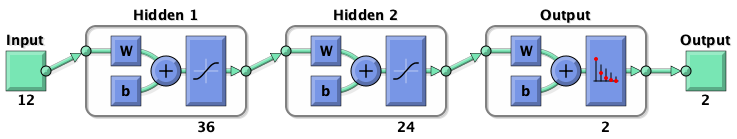
\includegraphics[width=0.7\linewidth]{neural.png}
 \captionof{figure}{Feed-forward neural network created.}
 \label{neural}
\end{minipage}
\\
\\
Note that the neural network created has 12 inputs and it outputs a $10000\times 2$ vector with the class prediction. The final step of the tuning process was selecting the activation and performance function. For the transfer function, the best results were encountered with the symmetric sigmoid transfer function \cite{matlab} in combination with the cross-entropy loss (logistic loss). The algorithm chosen for training was the scaled conjugate gradient backpropagation \cite{matlab2}, and the neural network converged with approximately 100 epochs.
\\
\\
The regularization parameter $\lambda$ of the loss function was set to 0.01 to present overfitting. Finally, we reserved 20\% of the training dataset for validation. The figure \ref{neural_training} shows the performance and the confusion matrix for the training dataset.
\\
\\
\begin{minipage}{\textwidth}
\centering
    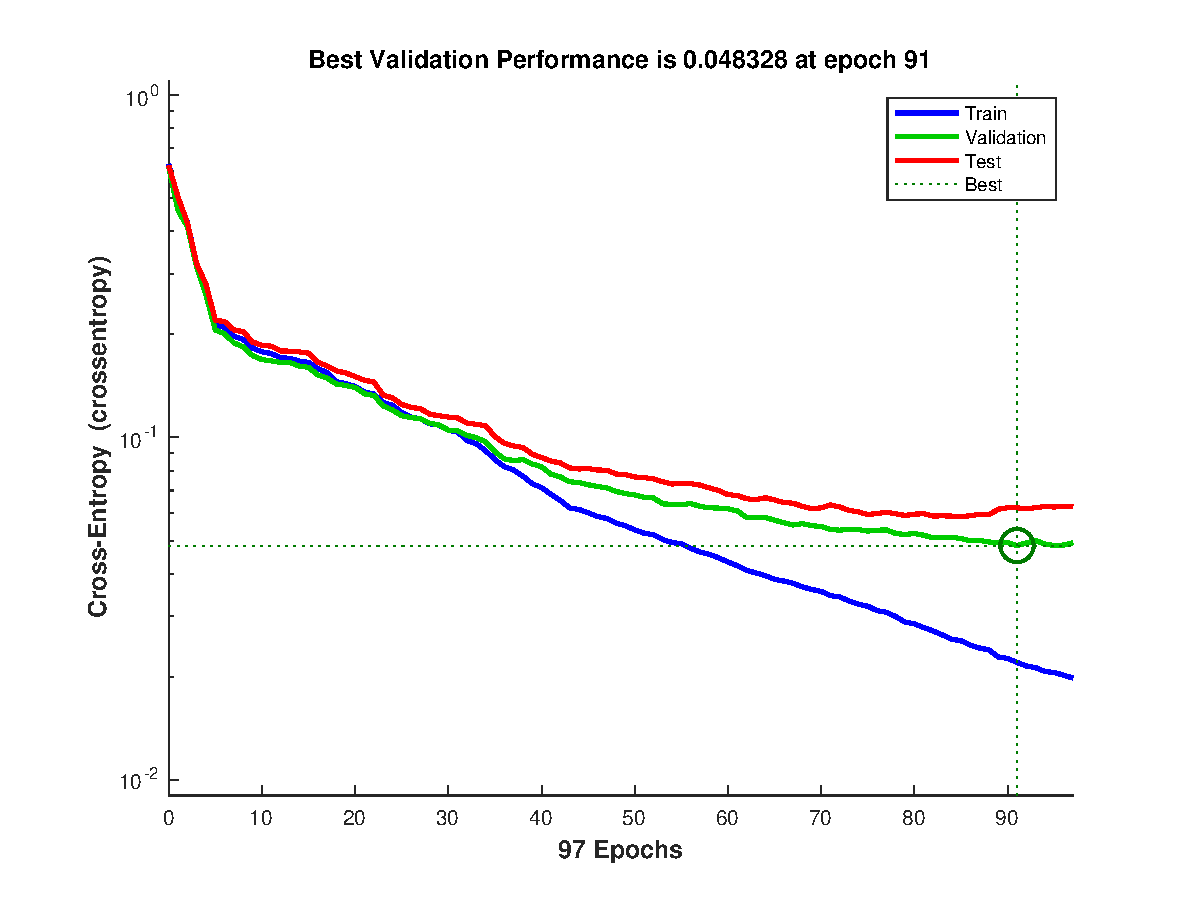
\includegraphics[width=0.4\linewidth]{chart_training.eps}
    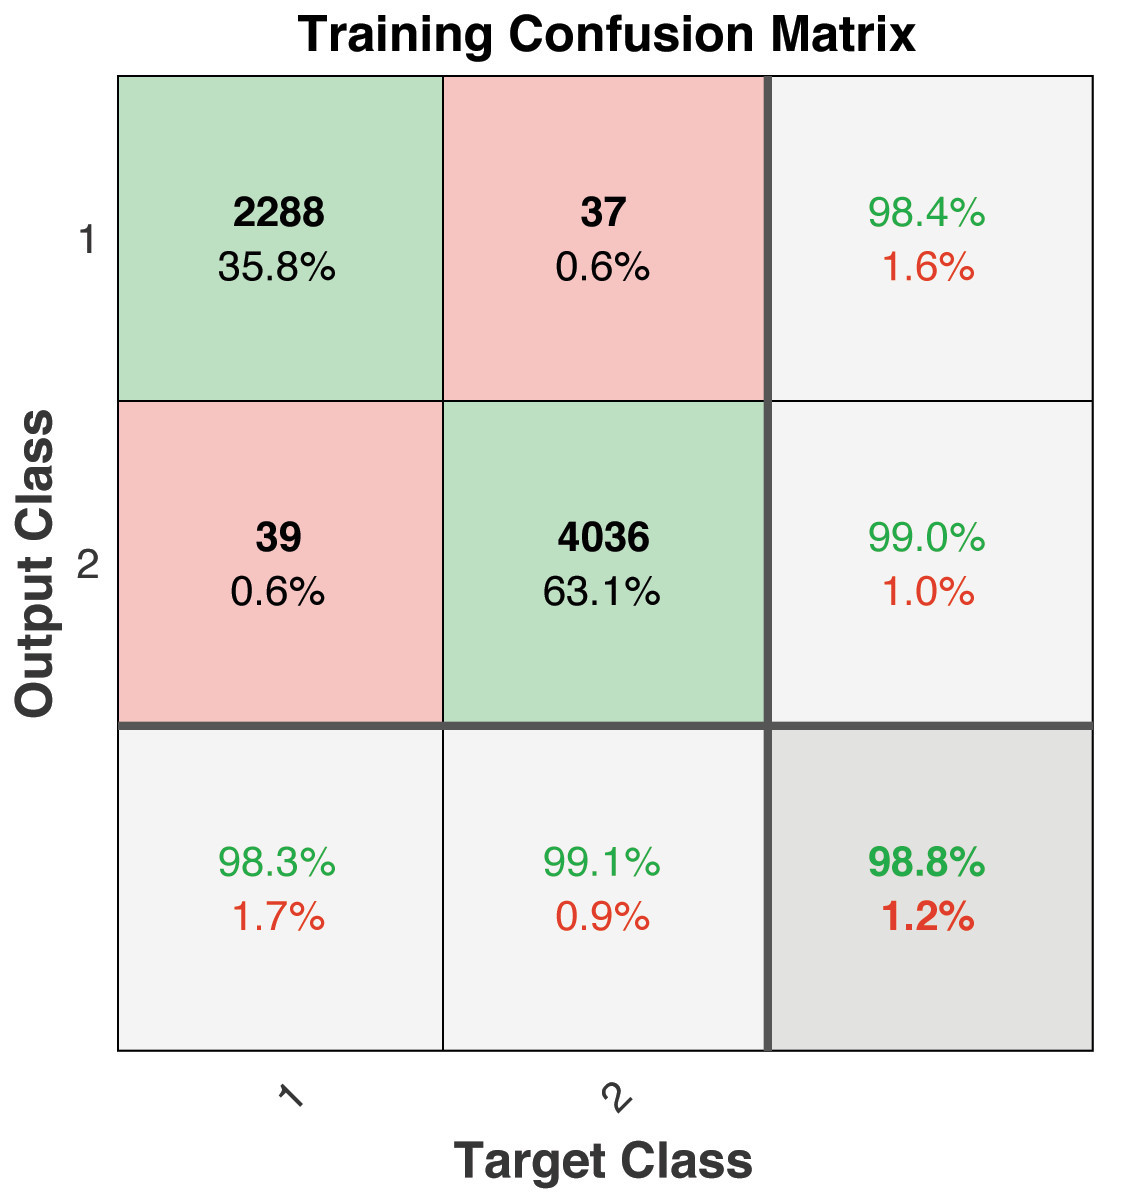
\includegraphics[width=0.28\linewidth]{matrix_nn.jpg}
 \captionof{figure}{Performance of the neural network on the left, and the confusion matrix on the training dataset only on the right (1 stands for stable and 2 for unstable).}
 \label{neural_training}
\end{minipage}
\\
\\
The F1-score of the training dataset is presented below.
\begin{gather*}
    F1_T = \frac{2\cdot TP}{2\cdot TP + FP + FN} = \frac{2\cdot 2288}{2\cdot 2288 + 39 + 37} = \boldsymbol{98.4\%}
\end{gather*}
When it comes to the F1-score on the validation dataset, we got $F1_{V} = 94.2\%$. Overall, this feed-forward neural network  demonstrated a promising performance over this dataset. 
\end{homeworkProblem}
\clearpage
% --------------------- Section 3 - not completed!
\begin{homeworkProblem}[Predictor \#2: k-nearest neighbour predictor]
The second predictor we trained was the k-nearest neighbour predictor. The process was completed in three steps: data preparation, parameter tuning and predictor evaluation.
\\
\\
First of all, we trained our first demo predictor using the training dataset based on the KNN Scikit Tool (with default parameters) in Python \cite{knn}. After testing the predictor on the training data, we saw that the accuracy at this stage was 86.2\%, which was not acceptable. So, we then tried a different range of k, from 1 to 50, and analyzed the results. The figure shows the results for the training dataset and the testing dataset using cross-validation. By observing the original data, we found that the range of each column in the input data are distinct, i.e., the range of tau1
(column 1) is around 0 to 10, and the range of g2 (column 10) is around 0 to 1. In this case, g2 may accidentally become more uninformative than tau1. This is because the calculation of distance in KNN is based on the input features, so a larger range feature has a larger impact on the distance since the Euclidian distance equation is given by $D(x,y) = \sqrt{\sum_n (x_i-y_i)^2}$. For this reason, we normalized all data by scaling them to the range of 0 to 1. 
\\
\\
Then we split the training dataset into training (80\%) and validation (20\%), and obtained an accuracy of 86.7\% on the validation dataset without any tuning. Next, we performed the parameter tuning step, which is one of the most important processes that dominate the behaviour of a predictor, and ultimately resulting in the best optimal combination of parameters possible. Although the Python sklearn’s documentation states there are eight parameters, we only put three of them into our tuning process:
\begin{itemize}
    \item \textit{n\_neighbours}: number of neighbours used to calculate k-neighbours. We tested from 2 to 20.
    \item  weights: there are two choices: uniform or distance. Uniform means all points in each neighbourhood are weighted equally whereas distance means the closer point is weighted more. We tested both cases.
    \item \textit{p}: Calculation procedure for the distance that the predictor will use:  1 for Manhattan distance, 2 for Euclidean distance and arbitrary number for Minkowski distance. We tried them all. 
\end{itemize}
We used 30 as the default size for the \textit{leaf\_size} variable (related to the construction time of the predictor), and the default algorithm for the distance metric used for the tree. 
\\
\\
Among all possible combinations, the one that had the best accuracy on training data was using  \textit{n\_neighbours = 16, weights = distance}, and \textit{p = 1}. The accuracy for this configuration was 87.9\% for the validation dataset and 98.7\% for the training dataset, which shows we did not overfit the data. We performed 10-fold cross-validation on the training dataset to avoid overfitting as much as possible, and the training and validation confusion matrices are presented in the figure \ref{neib}.
\\
\\
\begin{minipage}{\textwidth}
\centering
    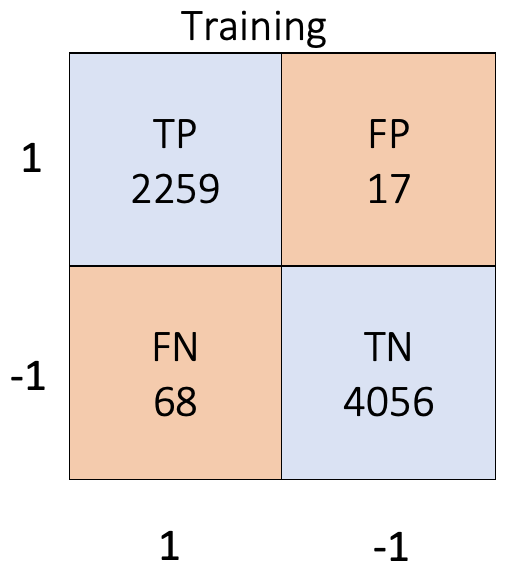
\includegraphics[width=0.2\linewidth]{train_m.png}
    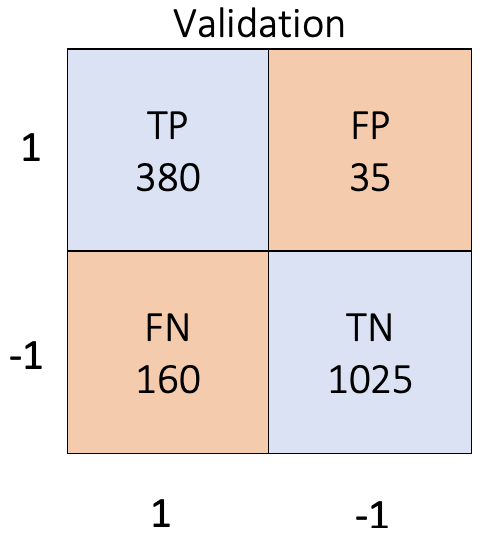
\includegraphics[width=0.2\linewidth]{valid_m.png}
 \captionof{figure}{ Confusion matrix of the training dataset on the left, and for the testing dataset on the right.}
 \label{neib}
\end{minipage}
\\
\\
We used the confusion matrix shown on figure \ref{neib} to calculate the F1-score for the training dataset.
\begin{gather*}
    F1_T = \frac{2\cdot TP}{2\cdot TP + FP + FN} = \frac{2\cdot 2259}{2\cdot 2259 + 17 + 68} = \boldsymbol{98.2\%}
\end{gather*}
When it comes to the F1-score on the validation dataset, we got $F1_{V} = 79.6\%$. In conclusion, the k-nearest neighbour predictor demonstrated satisfactory results in the training dataset.
\end{homeworkProblem}
\clearpage
% --------------------- Section 4
\begin{homeworkProblem}[Predictor \#3: kernelized support vector machine]
The third predictor we trained was the kernelized support vector machine (KSVM). To train and optimize the hyperparameters for the KSVM, we chose to use the classification learner toolbox in MATLAB \cite{matlab2}. Before training the predictor itself, we decided to use 5-fold cross-validation as a measure to prevent overfitting and to ensure we achieve a reliable predictor. This trade-off came at the expense of extra computing time when compared to using a holdout dataset. 
\\
\\
After directly importing our training dataset into MATLAB, we had several options to go about training the model. The first one was the type of kernel to be used; we could either use the gaussian or polynomial kernels of degree N. Then, there were the hyperparameters that we could change which consisted of the box constraint for all kernels, the degree of polynomial for polynomial kernels, the kernel scale for gaussian kernels, and finally whether to normalize our input data. From there, we trained and cross-validated several models using linear, quadratic, cubic, and fine/medium/coarse gaussian kernels. After analyzing the results, we noticed that a cubic kernel outperformed the other kernels. To validate our findings, we then ran a Bayesian optimizer for 10 iterations to seek out the best hyperparameters that were previously mentioned.
\\
\\
\begin{minipage}{\textwidth}
\centering
    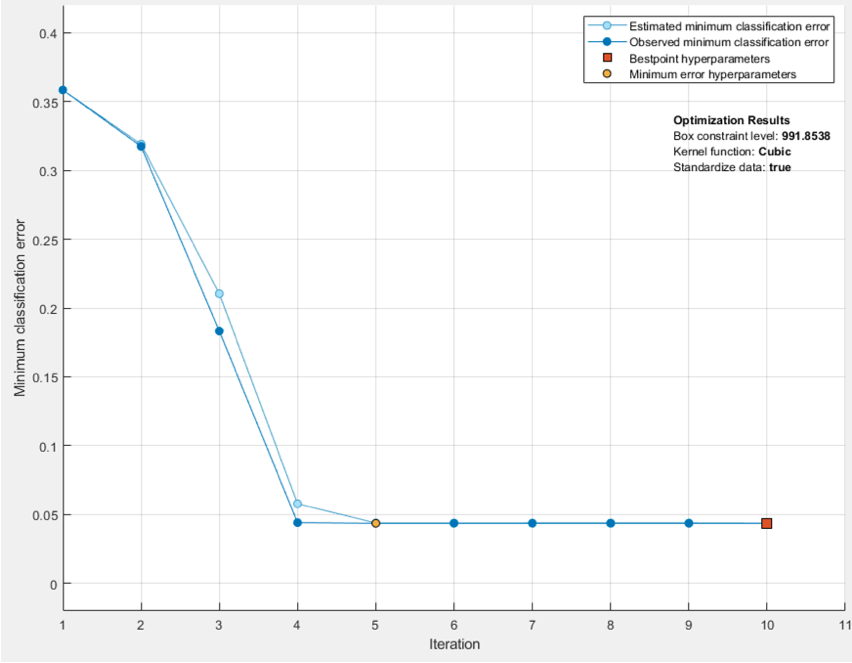
\includegraphics[width=0.4\linewidth]{ks_1.png}
 \captionof{figure}{Hyperparameter optimization iterations process to achieve the lowest cross-validation loss.}
 \label{ks1}
\end{minipage}
\\
\\
This combination of the cubic kernel with a box constraint of 991.85, and normalized input data led to the best performance with the accuracy of 98.9\%. Since this result was satisfactory, we then ran our predictor on the training and testing datasets to calculate the confusion matrices as shown in the figure \ref{ks2}.
\\
\\
\begin{minipage}{\textwidth}
\centering
    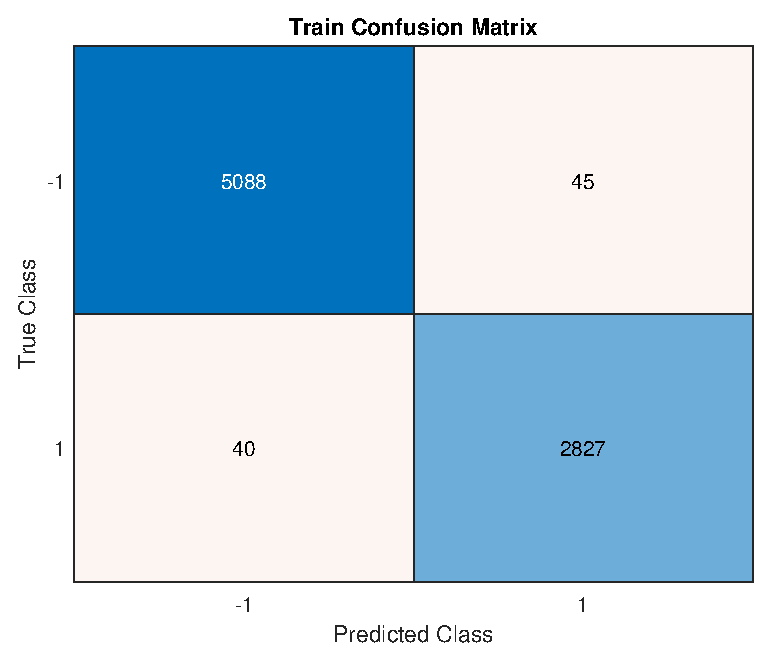
\includegraphics[width=0.3\linewidth]{trainmat.eps}
 \captionof{figure}{Confusion matrix of the training dataset.}
 \label{ks2}
\end{minipage}
\\
\\
From the confusion matrix in the figure \ref{ks2}, we can calculate the F1-score on the training dataset as follows:
\begin{gather*}
    F1_T = \frac{2\cdot TP}{2\cdot TP + FP + FN} = \frac{2\cdot 2827}{2\cdot 2827 + 45 + 40} = \boldsymbol{98.5\%}
\end{gather*}
From our results of a high cross-validation accuracy of 98.9\% and an F1-score of 98.5\% on our training data, it seems that our KSVM predictor achieves promising performance with little signs of overfitting.
\end{homeworkProblem}
\clearpage
% --------------------- Section 5
\begin{homeworkProblem}[Ensemble Learning]
In this section, we have evaluated the three predictors on the test set. We also tried weighted majority voting for ensemble learning. For this purpose, we have used the prediction vector generated on the test set by each predictor. We have used Python and scikit learn for this task \cite{knn}.
\\
\\
\textbf{Standalone model accuracy and F1-score:}
\\
For each predictor, the accuracy and F1-score for the test set can be seen in the table below:

\begin{center}
\begin{tabular}{@{}lll@{}}
\textbf{Predictor} & \textbf{Accuracy} & \textbf{F-1 Score}\\
\hline
Feed Forward Neural Network &	0.9545	&0.939\\
KNN &	0.861 &	0.7903                        \\
\textbf{Kernelized SVM} &	\textbf{0.963}	 & \textbf{0.9506}  
\end{tabular}
\end{center}

We can see that kernelized SVM outperforms the rest of the predictors on the test set. The second best performance is shown by the neural network. KNN seems to have the least accuracy and F1 score on the test set. 
\\
\\
\textbf{Weighted majority voting:}
\\
We combined the predictors using weighted majority hard voting. Each predictor was assigned a weight and all these predictions were combined by calculating dot product between assigned weight vector and prediction vector. We also created a grid search function to find a combination of weights that outputs the highest accuracy and F1-score. The results of some of the weights can be seen below:

\begin{center}
\begin{tabular}{@{}lll@{}}
\textbf{Weights [Predictor 1, Predictor 2, Predictor 3]} & \textbf{Accuracy} & \textbf{F-1 Score}\\
\hline
[0.333,0.333,0.333] &	0.9595	&0.9449\\
\textbf{[0.25, 0.25, 0.5],[0.3,0.2,0.5]} &	\textbf{0.965} &	\textbf{0.9538}     \\
{[0.5,0,0.5]} &    0.963   &0.952    \relax

\end{tabular}
\end{center}

The first row  shows results of assigning equal weights to all predictors. We see that the F1-score and accuracy is still less than standalone kernelized SVM. Second and third row show us weights generated by grid search which yield the best result. This is slightly higher than our best performing model (Kernelized SVM). Hence, we can see that ensemble learning can help in improving performance.

\end{homeworkProblem}
\begin{homeworkProblem}[Results]
The F1-score was used to evaluate the weighted average of precision and recall for the \textbf{feed-forward neural network} over this dataset due to the uneven class distribution. Applying the formula for the F1-score for the training, validation, testing, and all confusion matrices we get 98.4\%, 94.2\%, \textbf{93.9\%}, and 96.8\% respectively. These values are reasonable as the F1-score of the validation confusion matrix is less than the F1-score of the training-confusion matrix after adjusting the weights of the neural network to prevent overfitting. The results of the F1-score for the test confusion matrix is relatively close to the validation confusion matrix which shows that the validation predictor was successful.
\\
\\
When evaluating the performance of the \textbf{kernelized support vector machine}, we had an F1-Score of 98.5\% and a 98.9\% accuracy for our training dataset. When using the trained model to predict the labels for the testing dataset we had set aside, we calculated a new F1-score of \textbf{95.1\%}. This result shows that the KSVM model performs well in predicting unseen data as careful thought went into ensuring that it did not overfit the training dataset.
\\
\\
On the other hand, even though the \textbf{k-nearest neighbour} predictor has shown an excellent accuracy on the training data, the results obtained on validation and testing were not as good as we expected. This is because the F1-score for the validation and testing dataset was only 79.6\% and \textbf{79\%}, respectively. When we compare these results to the training dataset (98.5\%), we can notice that the true performance was far lower than the one obtained when training the predictor. One of the reasons for such a low performance can be overfitting during the training process. Therefore, predictor 2 did not perform as well as the others we trained. 



\end{homeworkProblem}
\clearpage

\newpage
\printbibliography


\end{document}
